\subsection{The Relational Model}

\textbf{\underline{Relation Schema}}
\bigskip
\begin{itemize}
    \item A \textbf{relation schema} R, denoted by $R(A_1,A_2,...,A_n)$, is made up of a relation name and a list of attributes.
    \item $attr(R)$ denotes the set of attributes of relation with name 
    \begin{itemize}
        \item[] $R$: $attr(Customer) = \underbrace{\{CustName, CustStreet, CustCity\}}_\text{Set}$
    \end{itemize}
\end{itemize}

\textbf{\underline{Attribute}}
\bigskip
\begin{itemize}
    \item The set of allowed values for each attribute is called the \textbf{domain} of the attribute
    \item Attribute values are required to be \textbf{atomic}; that is, indivisible
\end{itemize}

\textbf{\underline{Example of a Relation}}
\bigskip
\begin{figure}[H]
\centering
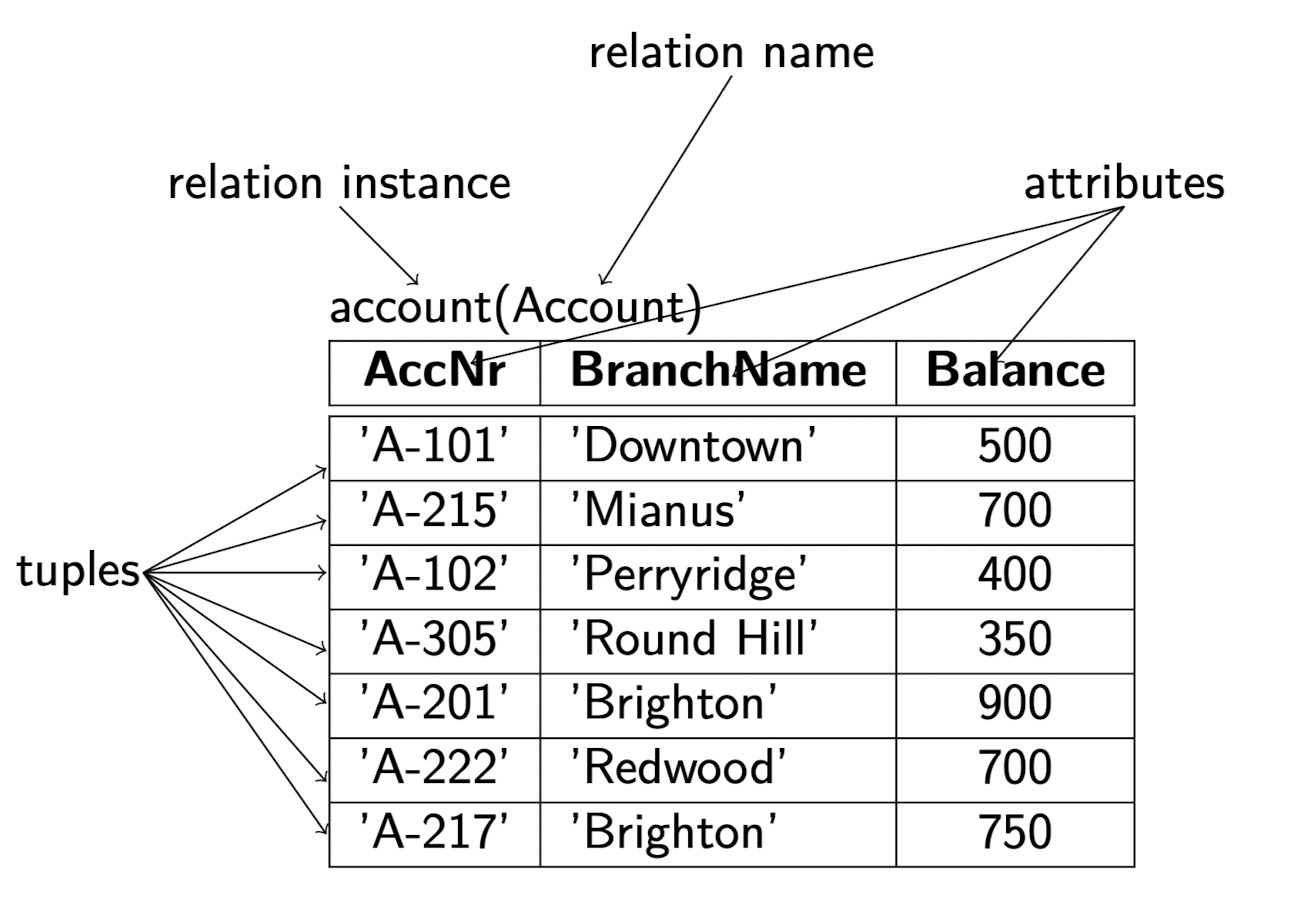
\includegraphics[width=0.8\textwidth]{images/Screenshot 2024-05-01 at 17.58.27.jpg}
\caption{Relation Example}
\end{figure}

\textbf{\underline{Characteristics of Relations}}
\bigskip
\begin{itemize}
    \item Relations are \textbf{unordered}, i.e., the order of tuples is irrelevant
\end{itemize}

\textbf{\underline{Database}}
\begin{itemize}
    \item A database consists of multiple relations
\end{itemize}

\textbf{\underline{Summary of the Relational Data Model}}
\begin{itemize}
    \item A \textbf{domain} $D$ is a set of atomic data values.
    \begin{itemize}
        \item phone numbers, names, grades, birthdates, departments
        \item each domain includes the special value \texttt{null}
    \end{itemize}
    \item With each domain a \textbf{data type} or format is specified.
    \begin{itemize}
        \item 5 digit integers, yyyy-mm-dd, characters
    \end{itemize}
    \item An \textbf{attribute} $A_i$ describes the role of a domain in a relation schema
    \begin{itemize}
        \item PhoneNr, Age, DeptName
    \end{itemize}
    \item A \textbf{relation schema} $R(A_1,...,A_n)$ is made up of a relation name $R$ and a list of attributes
    \begin{itemize}
        \item $Employee(Name,Dept,Salary),\ Departement(DName, Manager, Address)$
    \end{itemize}
    \item A \textbf{tuple} $t$ is an ordered list of values $t=(v_1,...,v_n)$ with $v_i \in dom(A_i)$
    \begin{itemize}
        \item $t=('Tom','SE',23K)$
    \end{itemize}
    \item A \textbf{relation} $r\subseteq D_1 \times ... \times D_n$ over schema $R(A_1,...,A_n)$ is a set of n-ary tuples
    \begin{itemize}
        \item $r= \{('Tom','SE',23K),('Lene','DB',33K)\}\subseteq Names \times Departments \times Integer$
        \item $s=\{('SE', 'Tom','Boston'),('DB','Lena','Tucson')\}$
    \end{itemize}
    \item A \textbf{database} $DB$ is a set of relations
    \begin{itemize}
        \item $DB=\{r,s\}$
    \end{itemize}
\end{itemize}

\textbf{\underline{Constraints}}
\bigskip
Key Constraints
\begin{itemize}
    \item Let $K\subseteq attr(R)$
    \item $K$ is a \textbf{superkey} of $R$ if values for $K$ are sufficient to identify a unique tuple of each possible relation $r$
    \item Superkey are not minimal
    \item $K$ is a \textbf{candidate key} if $K$ is minimal
    \item \textbf{Primary key}: a candidate key chosen as the principal means of identifying tuples within a relation
\end{itemize}
Entity constraints
\begin{itemize}
    \item The entity constraint requires that the primary key attributes of each relation may not have \texttt{null} values
\end{itemize}
\textbf{\underline{Referential Integrity}}
\bigskip
\begin{itemize}
    \item A relation schema may have an attribute that corresponds to the primary key of a relation. The attribute is called a \textbf{foreign key}.
\end{itemize}

\subsection{Basic Relational Algebra Operators}

\textbf{\underline{Basic Operators}}:
\begin{itemize}
    \item Select $\sigma$
    \item Project $\pi$
    \item Union $\cup$
    \item Set difference $-$
    \item Cartesian product $\times$
    \item Rename $\rho$
\end{itemize}

Relational algebra is a procedural language, i.e., order of operation matters

\subsubsection{Select Operator}
\begin{itemize}
    \item \textbf{Notation}: $\sigma_p(r)$
    \item $p$ is called the \textbf{selection predicate}
    \item \textbf{Definition}: $t\in \sigma_p(r) \Leftrightarrow t \in r \land p(t)$
    \item $p$ is a condition in propositional calculus consisting of \textbf{terms} connected by: $\land$ (\textbf{and}), $\lor$ (\textbf{or}), $\lnot$ (\textbf{not})
    \item Example: $\sigma_{A=B\land D >5}(r)$
\end{itemize}

\subsubsection{Project Operator}
\begin{itemize}
    \item \textbf{Notation}: $\pi_{A_1,...,A_k}(r)$
    \item The result is defined as the relation of $k$ columns obtained by deleting the columns that are not listed
    \item \textbf{Definition}: $t\in \pi_{A_1,...,A_k}(r) \Leftrightarrow \exists x(x\in r \land t = x[A_1,...,A_k])$
    \item There are no duplicate rows in the result since relations are sets
    \item Example: $\pi_{A,C}(r)$
\end{itemize}

\subsubsection{Union Operator}
\begin{itemize}
    \item \textbf{Notation}: $r \cup s$
    \item \textbf{Definition}: $t\in (r\cup s) \Leftrightarrow t \in r \lor t \in s$
    \item For $r\cup s$ to be valid $r$ and $r$ must have union compatible schema
    \item Example: $r \cup s$
\end{itemize}

\subsubsection{Set Difference Operator}
\begin{itemize}
    \item \textbf{Notation}: $r-s$
    \item \textbf{Definition}: $t\in (r-s) \Leftrightarrow t \in r \land t \notin s$
    \item Set differences must be taken between (union) compatible relations.
    \item Example: $r-s$
\end{itemize}

\subsubsection{Cartesian Product Operator}
\begin{itemize}
    \item \textbf{Notation}: $r \times s$
    \item \textbf{Definition}: $t \in (r \times s) \Leftrightarrow x \in r \land y \in s \land t = x \circ y$
    \item The attribute names of $r$ and $s$ must be disjoint, otherwise a naming conflict exists. To prevent naming conflict, renaming must be used.
    \item Example: $r \times s$
\end{itemize}

\begin{figure}[H]
\centering
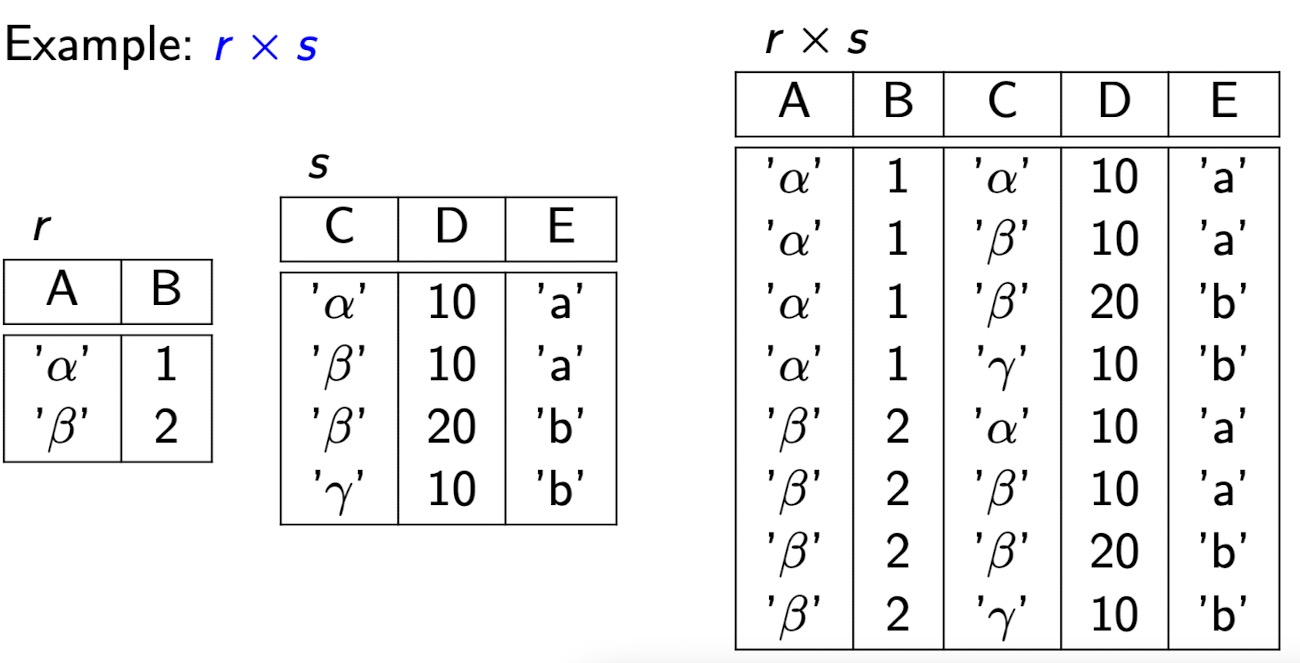
\includegraphics[width=0.6\textwidth]{images/Screenshot 2024-05-01 at 18.40.41.jpg}
\caption{Cartesian Product}
\end{figure}

\subsubsection{Rename Operator}
\begin{itemize}
    \item Allows us to name the results of relation algebra expressions by setting relation and attribute names
    \begin{itemize}
        \item $\rho_r(E)$ changes the relation name to $r$
        \item $\rho_{r(A_1,...,A_n)}(E)$ changes the relation name to $r$ and the attribute names to $A_1,...,A_k$
        \item $\rho_{(A_1,...,A_n)}(E)$ changes attribute names to $A_1,...,A_k$
    \end{itemize}
    \item Example: $\rho_{s(X,Y,U,V)}(r)$
\end{itemize}

\subsection{Additional Relational Algebra Operators}

\begin{itemize}
    \item Set intersection $\cap$
    \item Join $\bowtie$
    \item Division $\div$
    \item Assignment $\leftarrow$
\end{itemize}

These additional operators \textbf{do not add expressive power}. They just simplify queries, they could be replaced by basic operators.

\subsubsection{Set Intersection Operator}
\begin{itemize}
    \item \textbf{Notation}: $r \cap s$
    \item \textbf{Definition}: $t \in (r \cap s) \Leftrightarrow t \in r \land t \in s$
    \item Precondition:
    \begin{itemize}
        \item $r,s$ have the same arity
        \item attributes of $r$ and $s$ are compatible
    \end{itemize}
    \item Note: $r \cap s = r-(r-s)$
    \item Example: $r \cap s$
\end{itemize}

\subsubsection{Theta Join Operator}
\begin{itemize}
    \item \textbf{Notation}: $r \bowtie_\theta s$
    \item \textbf{Definition}: Let $r$ and $s$ be relations on schema $R$ and $S$, respectively. $\theta$ is a boolean condition on the attributes of $r$ and $s$
    \item $r \bowtie_\theta s$ is a relation on schema that includes all attributes from schema $R$ and all attributes from schema $S$
    \item Example: $r \bowtie_{B<X\land D = Y} \rho_{(X,Y,Z)} (s)$
\end{itemize}

\subsubsection{Natural Join Operator}
\begin{itemize}
    \item \textbf{Notation}: $r \bowtie s$
    \item \textbf{Definition}: Let $r$ and $s$ be relations on schema $R$ and $S$, respectively.
    \item $r \bowtie s$ is a relation on schema that includes all attributes from schema $R$ and all attributes from schema $S$ that do not occur in schema $R$.
    \item Example: $r \bowtie (s)$ [works only if attribute names are the same]
\end{itemize}

\subsubsection{Division Operator}
\begin{itemize}
    \item \textbf{Notation}: $r \div s$
    \item Suited for queries that include the phrase "for all".
    \item Let $r$ and $s$ be relations on schemas $R(A_1,...,A_m,B_1,...,B_n)$ and $S(B_1,...,B_n)$, respectively.
    \item The result of $r \div s$ is a relation with attributes $R-S=(A_1,...,A_m)$
    \item \textbf{Definition}: $t\in (r \div s) \Leftrightarrow t \in \pi_{R-S}(r) \land \forall u \in s(t\circ u \in r)$
    \begin{itemize}
        \item $t \circ u$ is the concatenation of tuples $t$ and $u$
        \item $R-S$: all attributes of schema $R$ that are not in schema $S$
    \end{itemize}
    \item Own words: $r\div s$ gives all tuples of $r$ (only those attributes that are not in $s$), where all possible combinbations with $s$ exists: 

\begin{figure}[H]
\centering
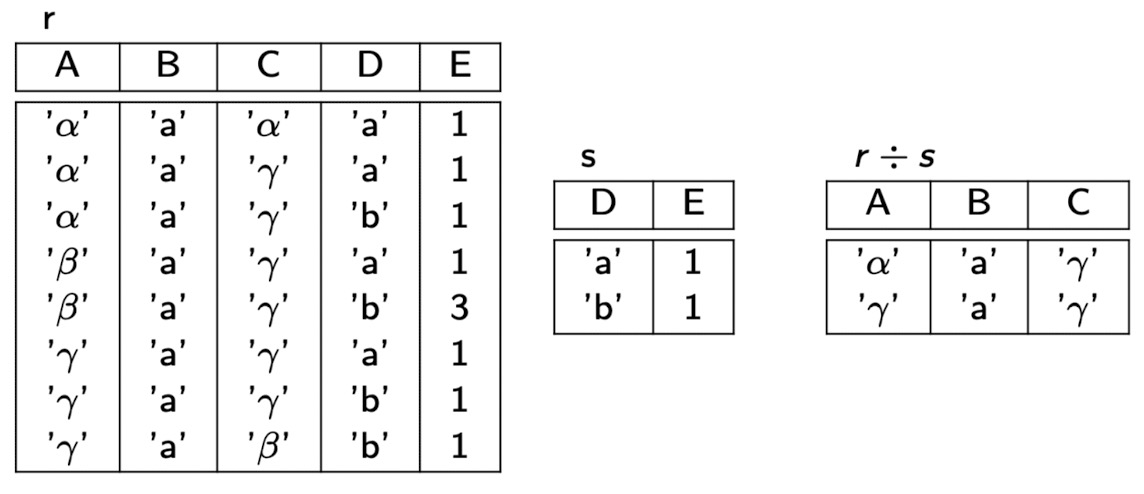
\includegraphics[width=0.6\textwidth]{images/Screenshot 2024-05-04 at 09.59.38.jpg}
\caption{Division Operator}
\end{figure}
    \begin{itemize}
        \item $'\alpha','a','\gamma'$ is in output because both 'combinations' with $s$, $'\alpha','a','\gamma','a',1$ and $'\alpha','a','\gamma','b',1$ exist already in $r$.
        \item $'\beta','a','\gamma'$ is not in output because only $'\beta','a','\gamma','a',1$ is in $r$ and $'\beta','a','\gamma','b',1$ is not
    \end{itemize}
    \item Property: 
    \begin{itemize}
        \item Let $q=r\div s$
        \item Then $q$ is the largest relation satisfying $q\times s \subseteq r$
    \end{itemize}
\end{itemize}

\subsubsection{Assignment Operator}
\begin{itemize}
    \item The assignment operator $\leftarrow$ provides a convenient way to express complex queries by breaking them up into smaller pieces
\end{itemize}

\subsection{Extended Relational Algebra Operators}

\subsubsection{Generalized Projection}
\begin{itemize}
    \item Extends the projection operation by allowing arithmetic functions to be used in the projection list
    \item Example: $\pi_{CustName, Limit - CreditBal}(credit_info)$
\end{itemize}
\subsubsection{Aggregate Functions}
\begin{itemize}
    \item \textbf{Aggregate function} takes a collection of values and returns a single value as a result: (avg, min, max, sum, count)
    \item Example: $res \leftarrow \rho_{Res(SumC)} ( \vartheta _{sum(C)} (r))$
    \item Example: $res \leftarrow \rho_{Res(BName,SumBal)}(_{BranchName} \vartheta_{sum(Balance)}(account))$, where $BranchName$ is a grouping criteria
\end{itemize}
\subsubsection{Outer Join}
\begin{itemize}
    \item The (inner) join does not return tuples that do not have a join partner.
    \item The outer join avoids this loss of information. (By using \texttt{null} values).
    \item \textbf{Left Outer Join} preserves tuples from the left table
    \item \textbf{Right Outer Join} preserves tuples from the right table
    \item \textbf{Full Outer Join} preserves all tuples
\end{itemize}

\subsection{Modification of the Database}
Modifications are done by using the assignment operator:
\begin{itemize}
    \item Delete: $r\leftarrow r - E$
    \item Insert: $r \leftarrow r \cup E$
    \item Update: $r \leftarrow E$
\end{itemize}
Modification operations are expensive, since space for the tuples must be allocated/deallocated.
\subsection{Relation Algebra Notation in Text Terminals}

\begin{figure}[H]
\centering
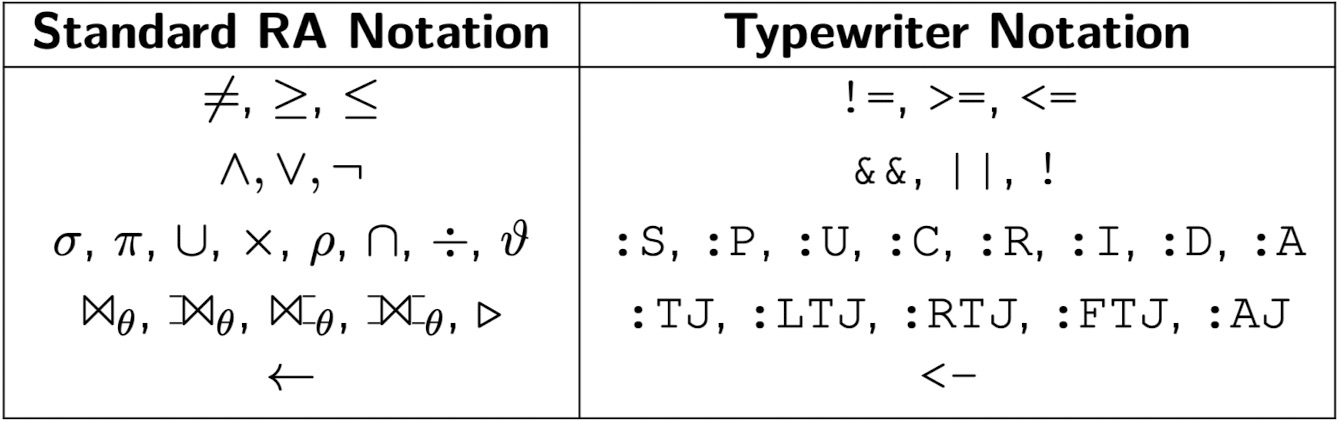
\includegraphics[width=0.6\textwidth]{images/Screenshot 2024-05-04 at 10.44.01.jpg}
\caption{Text Terminal Notation}
\end{figure}
\begin{itemize}
    \item Additional Typewriter Notation for DRC:
    \begin{itemize}
        \item $\Rightarrow=$ \texttt{=>}
        \item $\forall=$ \texttt{:F}
        \item $\exists$ \texttt{:E}
    \end{itemize}
    \item Instead of subscripts use \texttt{[ ]} brackets
    \item Replace \texttt{T} with \texttt{N} for natural joins
\end{itemize}

\subsection{Relational Calculus}

Relational calculus is a \textbf{non-procedural} or \textbf{declarative} language

\subsubsection{First Order Predicate Logic}
Syntax:
\begin{itemize}
    \item \textbf{logical symbols}: $\land, \lor, \lnot, \Rightarrow, \exists, \forall, ...$
    \item \textbf{constant}: string, number,...;
    \item \textbf{identifier}: character sequence starting with a letter
    \item \textbf{variable}: identifier starting with capital letter
    \item \textbf{predicate symbol}: identifier starting with lower case letter
    \item \textbf{built-in predicate symbol}: $=,<,>,\leq,\geq,\neq,...$
    \item \textbf{term}: constant, variable
    \item \textbf{atom}: predicate, built-in predicate; $p(t_1,...,t_n), t_1<t_2,...$ with terms $t_1,...,t_n$; predicate symbol $p$
    \item \textbf{formula}: atom, $A \land B, A \lor B, \lnot A, A \Rightarrow B, \exists XA, \forall XA, (A),... $ with formulas $A, B$; variable $X$
\end{itemize}
Terminology:
\begin{itemize}
    \item A variable is \textbf{free} is it is not quantified
    \item A variable is \textbf{bound} if it is quantified
\end{itemize}

\subsubsection{Domain Relation Calculus}
A domain relational calculus query is of the form $\{X_1,...,X_n | formula \}$, where $X_1,...,X_n$ are the only free variables in \textit{formula}
\begin{itemize}
    \item Example: To determine first and last names of all employees whose salary is above \$50,000, we write: \[
    \{FN, LN \ |\  \exists Sal(emp(FN, \_, LN, \_, Sal) \land Sal >50000) \}
    \]
\end{itemize}